\chapter{Implémentation et résultats}
\begin{figure*}[h!]

   \centering
   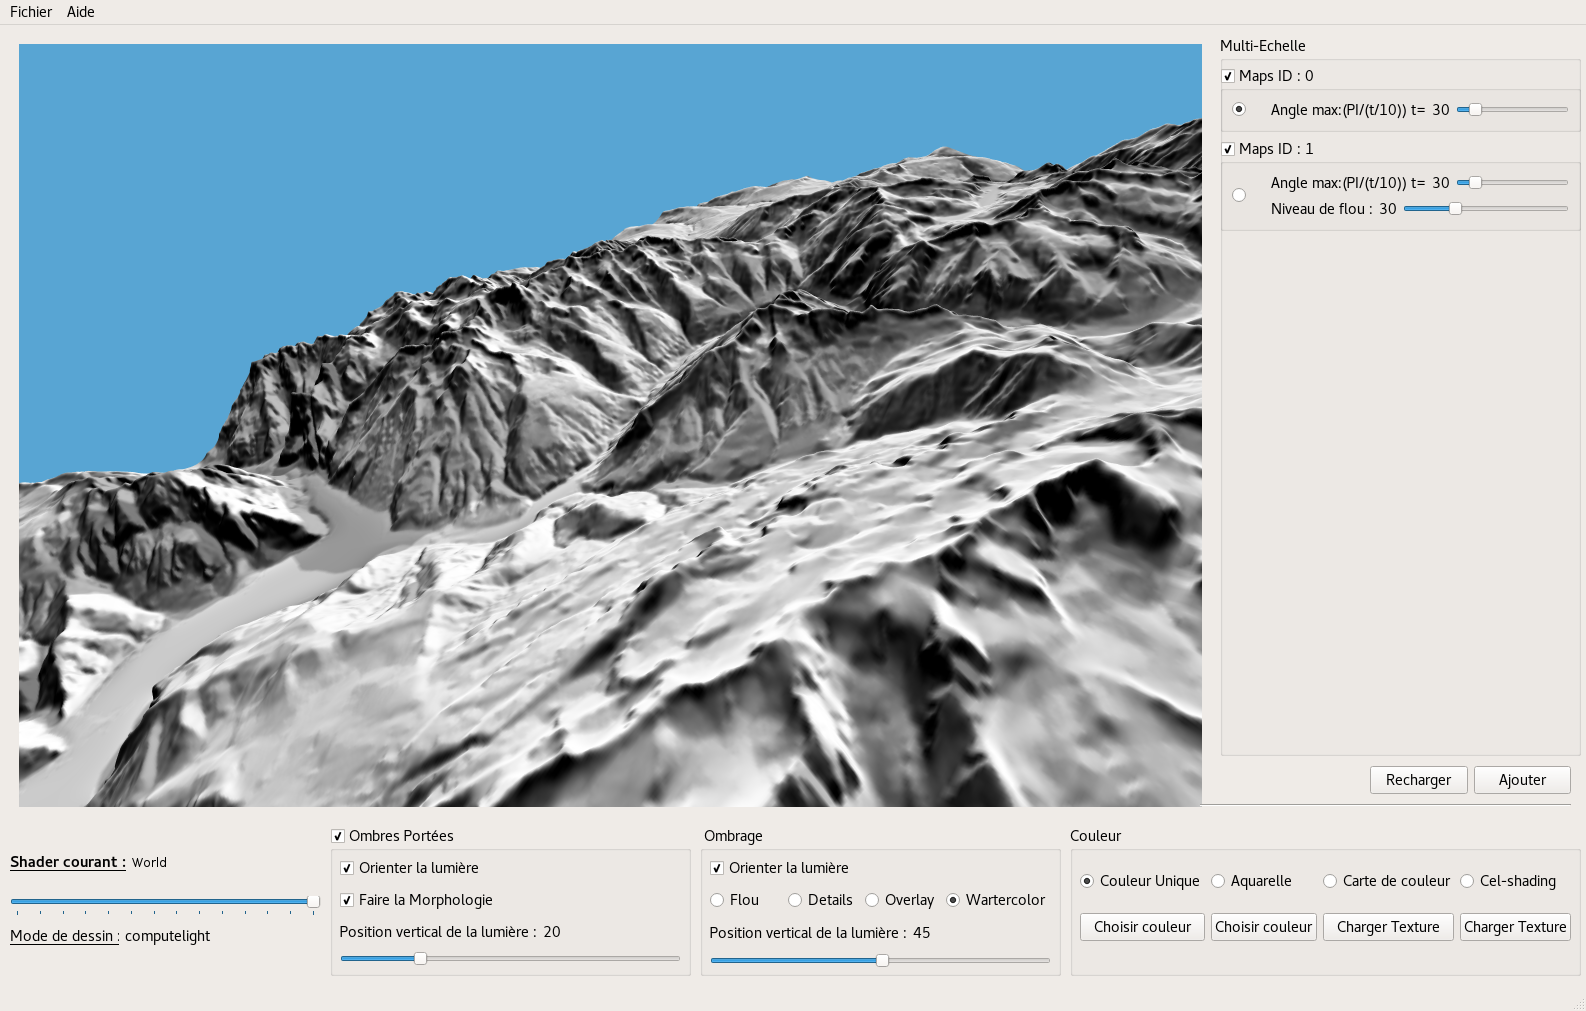
\includegraphics[width=1.0\linewidth]{Resultats/interface.png}
   \caption{Interface de notre prototype}
\end{figure*}

\section{Degrés de libertés}
Dans notre implémentation, nous avons fait le choix de laisser des paramètres que l'utilisateur peut modifier  afin d'être plus proche de ce que pourrait donner un logiciel de rendu de panorama "à la Novat". Dans un premier temps, il peut choisir un ou plusieurs MNT (à condition qu'ils soient continus et que la carte reste rectangulaire). Pour modifier le rendu des ombres, il peut modifier les paramètres de l'ombrage (élévation de la lumière et orientation ou non de la lumière), des ombres portées (élévation de la lumière, orientation ou non de la lumière et abstraction ou non des formes), du multi-echelle (quantité de flou, manière de fusionner les ombrages) et de mise en couleur (unie, aquarelle, carte de couleur ou cel-shading). 
\section{Implémentation}
Notre système de rendu est implémenté en C++ 14 et QT 5.10. Le rendu en lui même est fait en OpenGL et GLSL 4.5 et la plupart des calculs sont faits sur GPU, dans les shaders, avec plusieurs passes successives.  La taille du widget de rendu 3D fait 1200*780 pixels. Notre rendu comprend une camera, une lumière,  ainsi qu'un maillage généré à partir d'un ou plusieurs modèles numériques de terrain (MNT). Pour notre rendu sur la région de l'Alpe d'Huez, nos données font $800*1200$ avec un pas de $25$m et donc couvrent $24$km$^2$, il en résulte un maillage de $5748006$ triangles. Avec une carte graphique \textit{NVIDIA Quadro 6000}, nous avons un rendu à $60$ images par seconde en moyenne sans les ombres portées, $20$ avec, ce qui permet d'avoir un logiciel interactif.  

\paragraph*{Modèle Numérique de Terrain (MNT) : } C'est une carte de hauteur sous la forme d'une dalle carrée de taille variable en fonction de son niveau de détail. Il y a $4$ niveaux de détails proposés par l'IGN : $75$m, $25$m, $5$m et $1$m qui représentent la distance entre chaque donnée. Ainsi une dalle avec un niveau de détail de $25$m fera $4$km$^{2}$, et une dalle avec un niveau de détail de 1m fera $1$km$^{2}$. Les MNT utilisés dans ce projet sont récupérés sur le site de l'Institut national de l'information géographique et forestière (IGN). Ce site permet d'obtenir un ensemble de dalles continues personnalisé.   




\section{Résultats}
Voici un ensemble de résultats que nous avons produits principalement sur le relevé topologique de la région l'Alpes d'Huez (6 dalles avec un niveau de détail de $25$m). $\alpha$ correspond à l'orientation de l'azimut de la lumière globale, $\gamma_o$  l'élévation de la lumière pour l'ombrage, $\gamma_p$ l'élévation de la lumière pour les ombres portées et $\sigma$ la quantité de flou appliqué sur la $2^e$ échelle.  

\begin{figure*}[h!]
\centering
 \begin{subfigure}[t]{0.32\linewidth}
 \centering
 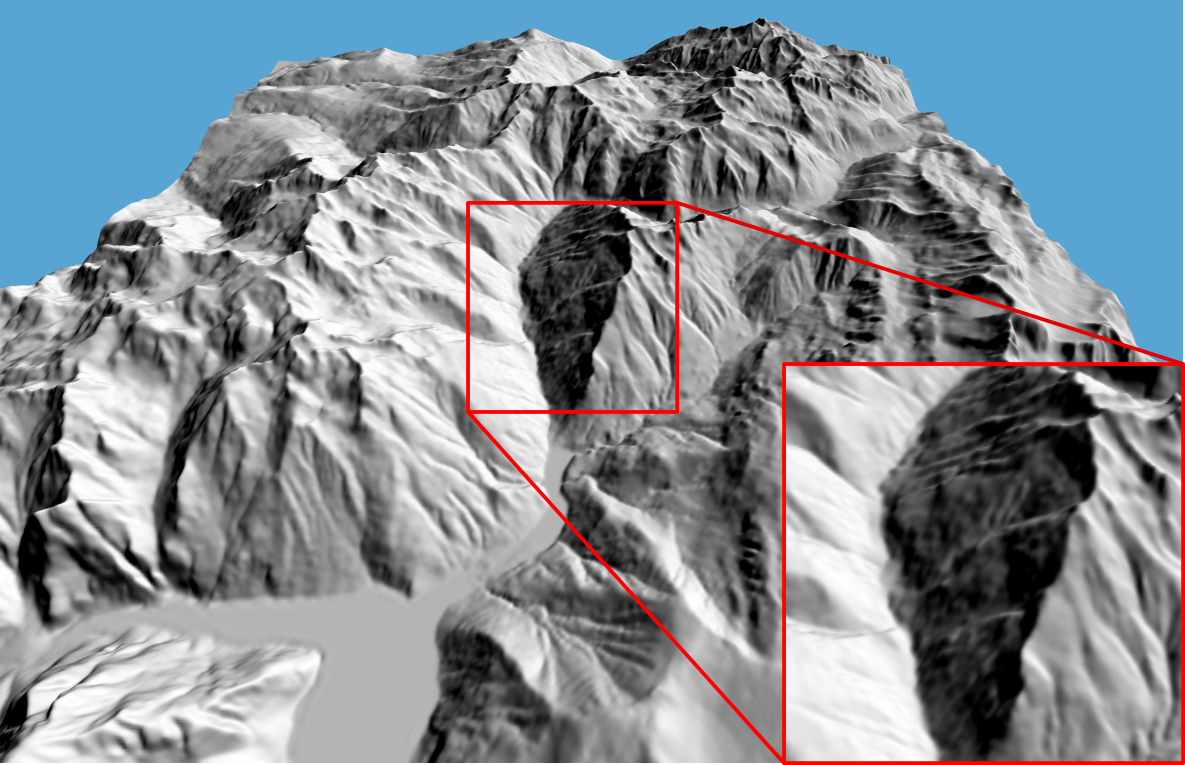
\includegraphics[width=1.0\linewidth]{Resultats/lambertien.png}
 \caption{Lambertien classique }
 \end{subfigure}
 \begin{subfigure}[t]{0.32\linewidth}
 \centering
 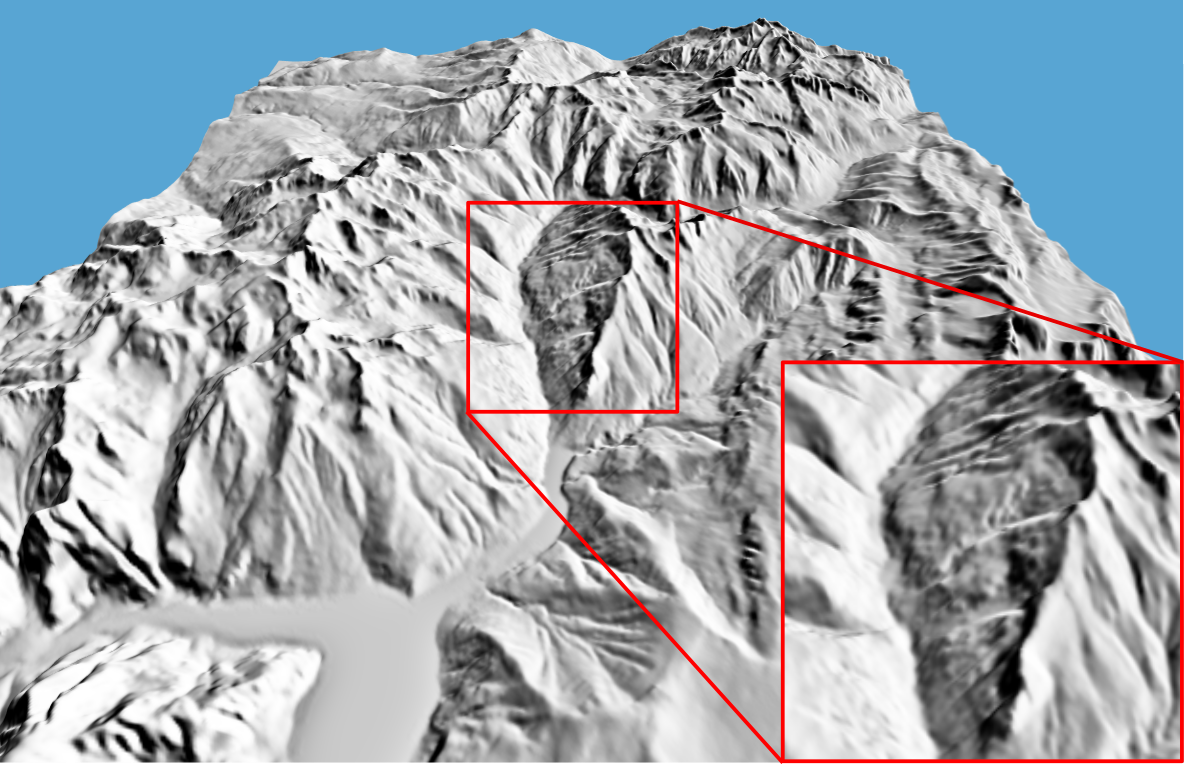
\includegraphics[width=1.0\linewidth]{Resultats/ombrage.png}
  \caption{Notre méthode}
 \end{subfigure}
  \begin{subfigure}[t]{0.32\linewidth}
 \centering
 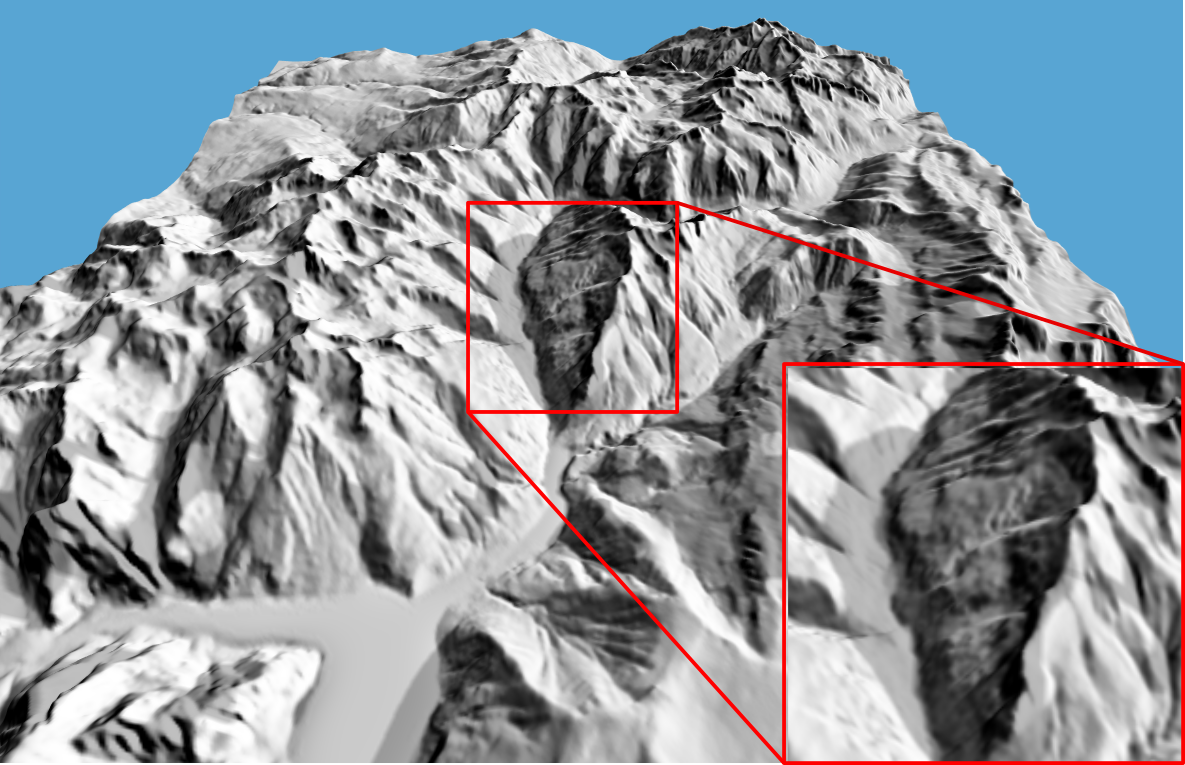
\includegraphics[width=1.0\linewidth]{Resultats/ombre_portee.png}
  \caption{Notre méthode avec les ombres portées}
 \end{subfigure}
 \caption{Comparaison de notre méthode avec un Lambertien classique ($\alpha = 270\degres$ (Est) $\gamma_o = 45\degres$ , $\gamma_p = 20\degres$, $\sigma = 30$).}
\end{figure*}



\begin{figure*}[h!]
\centering
 \begin{subfigure}[t]{0.24\linewidth}
   \centering
   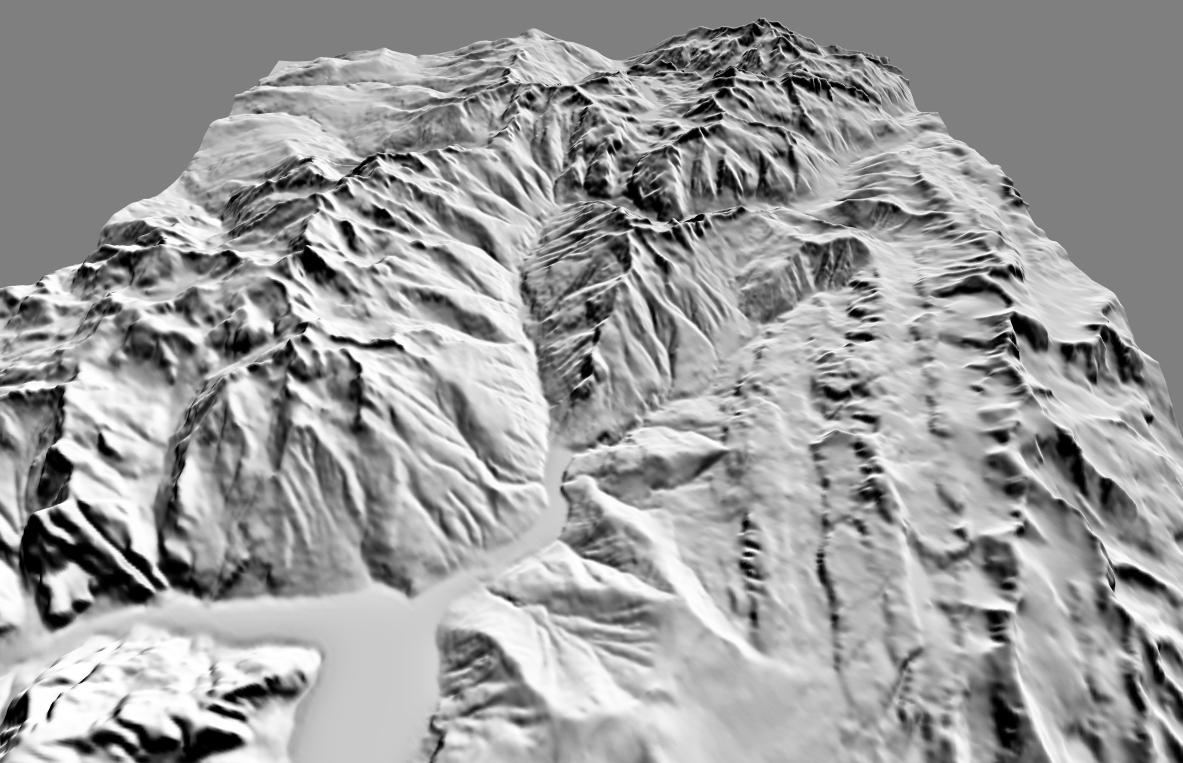
\includegraphics[width=1.0\linewidth]{Resultats/2_nord_our.png}
   \caption{$\alpha = 0\degres$ (Nord)}
 \end{subfigure}
 \begin{subfigure}[t]{0.24\linewidth}
   \centering
   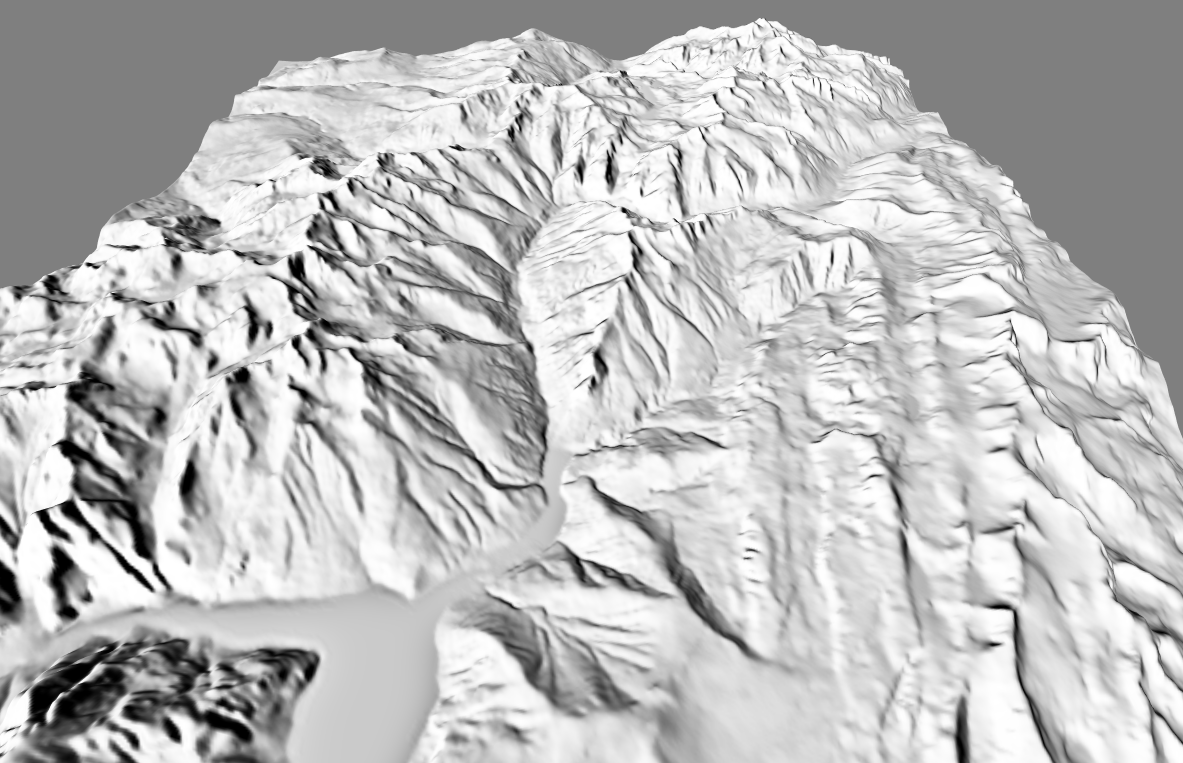
\includegraphics[width=1.0\linewidth]{Resultats/2_sud_our.png}
   \caption{$\alpha = 180\degres$ (Sud)}
 \end{subfigure}
 \begin{subfigure}[t]{0.24\linewidth}
   \centering
   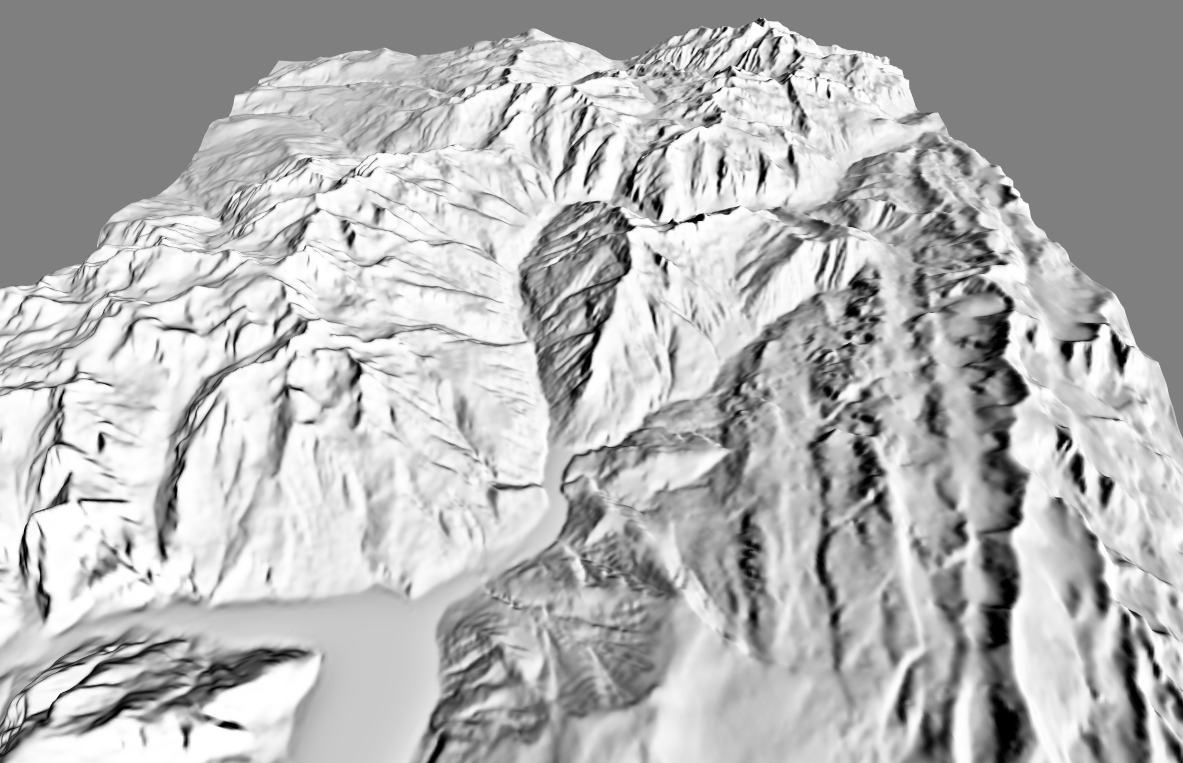
\includegraphics[width=1.0\linewidth]{Resultats/2_est_our.png}
   \caption{$\alpha = 270\degres$ (Est)}
 \end{subfigure}
 \begin{subfigure}[t]{0.24\linewidth}
   \centering
   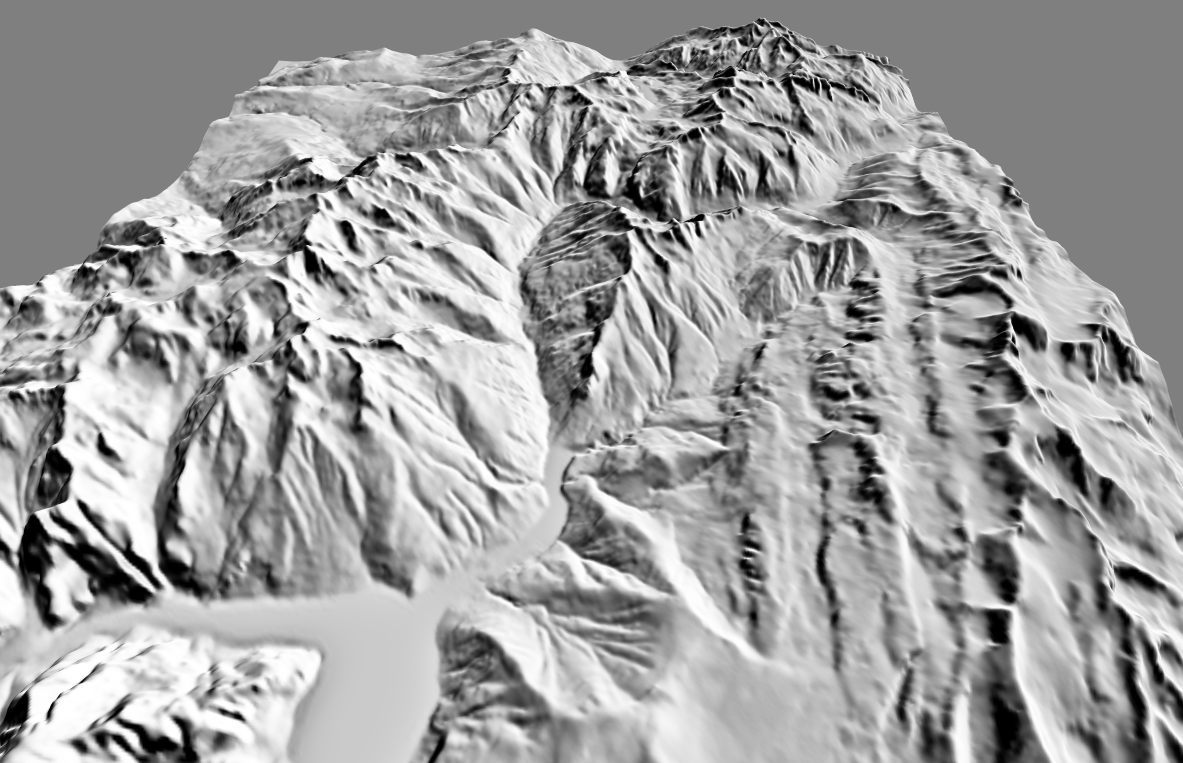
\includegraphics[width=1.0\linewidth]{Resultats/2_nordest_our.png}
   \caption{$\alpha = 315\degres$ (Nord-Est)}
 \end{subfigure}
  \begin{subfigure}[t]{0.24\linewidth}
   \centering
   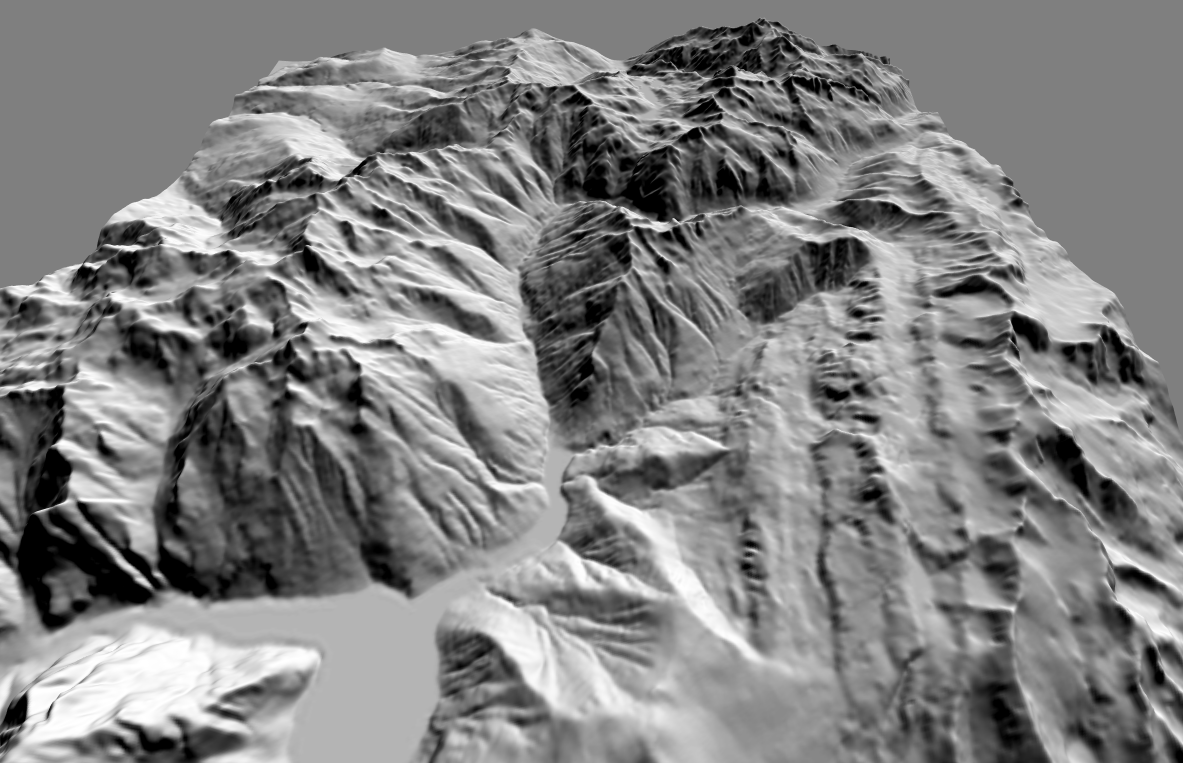
\includegraphics[width=1.0\linewidth]{Resultats/2_nord_lambert.png}
   \caption{$\alpha = 0\degres$ (Nord)}
 \end{subfigure}
 \begin{subfigure}[t]{0.24\linewidth}
   \centering
   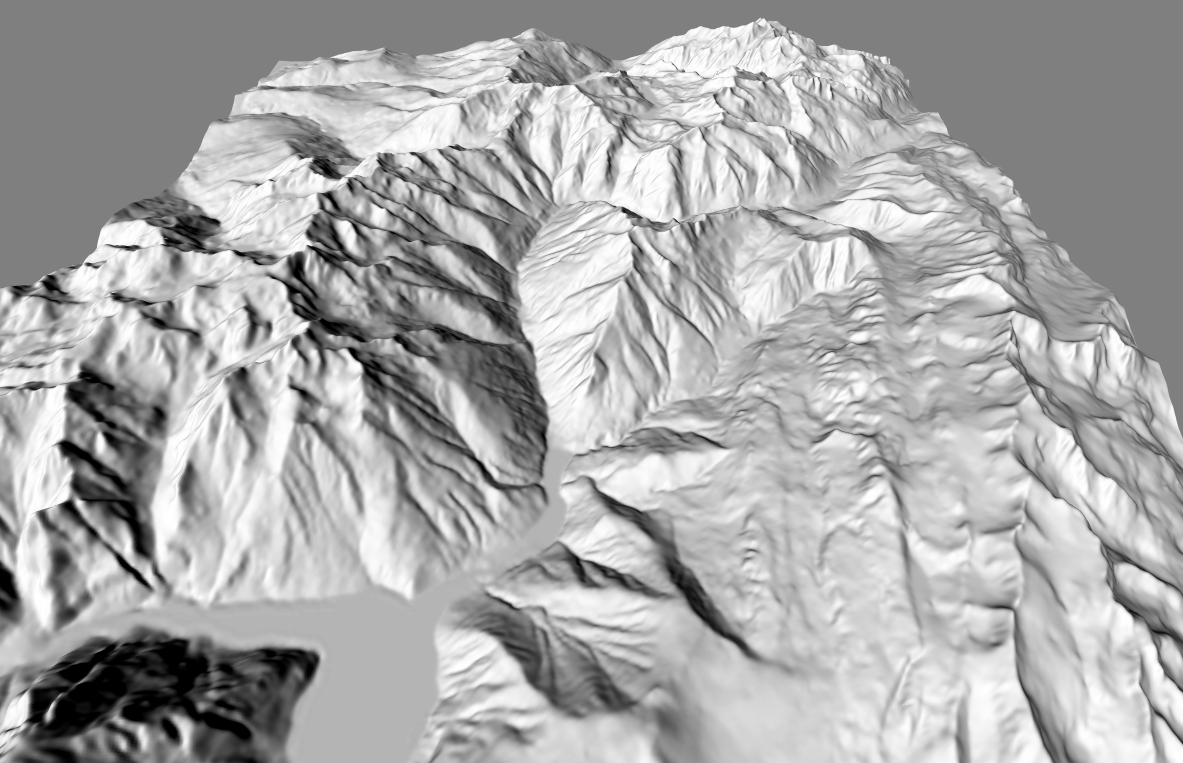
\includegraphics[width=1.0\linewidth]{Resultats/2_sud_lambert.png}
   \caption{$\alpha = 180\degres$ (Sud)}
 \end{subfigure}
 \begin{subfigure}[t]{0.24\linewidth}
   \centering
   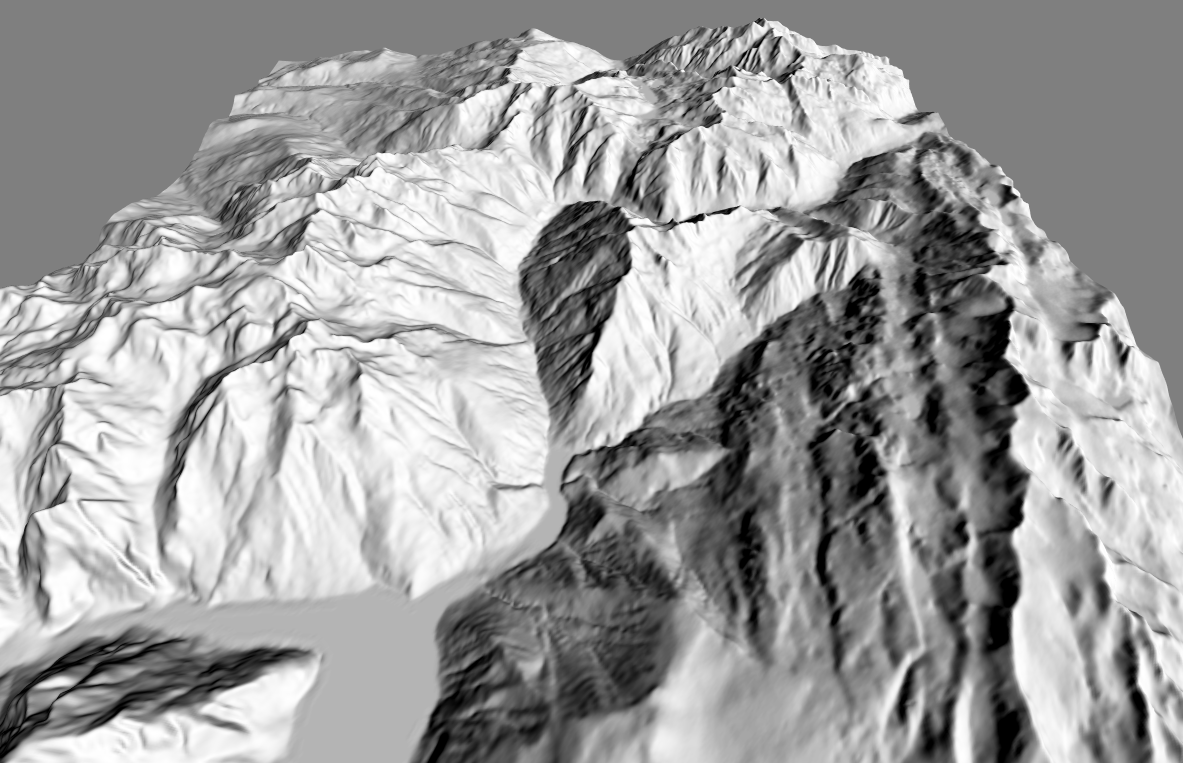
\includegraphics[width=1.0\linewidth]{Resultats/2_est_lambert.png}
   \caption{$\alpha = 270\degres$ (Est)}
 \end{subfigure}
 \begin{subfigure}[t]{0.24\linewidth}
   \centering
   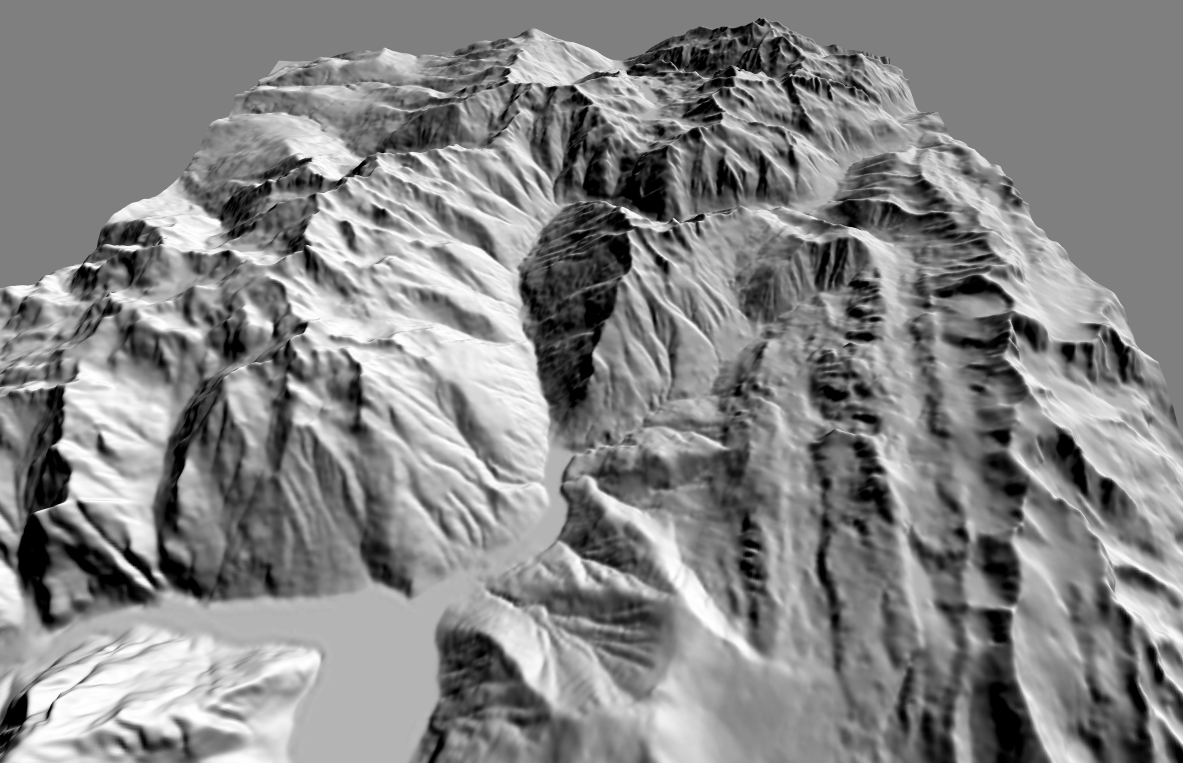
\includegraphics[width=1.0\linewidth]{Resultats/2_nordest_lambert.png}
   \caption{$\alpha = 315\degres$ (Nord-Est)}
 \end{subfigure}
 \caption{Comparaison entre notre méthode (ligne du haut) et un Lambertien classique (ligne du bas) avec plusieurs orientations du soleil. ( $\gamma_o = 45\degres$ , $\sigma = 30$)}
\end{figure*}


\begin{figure*}[h!]
\centering
 \begin{subfigure}[t]{0.24\linewidth}
   \centering
   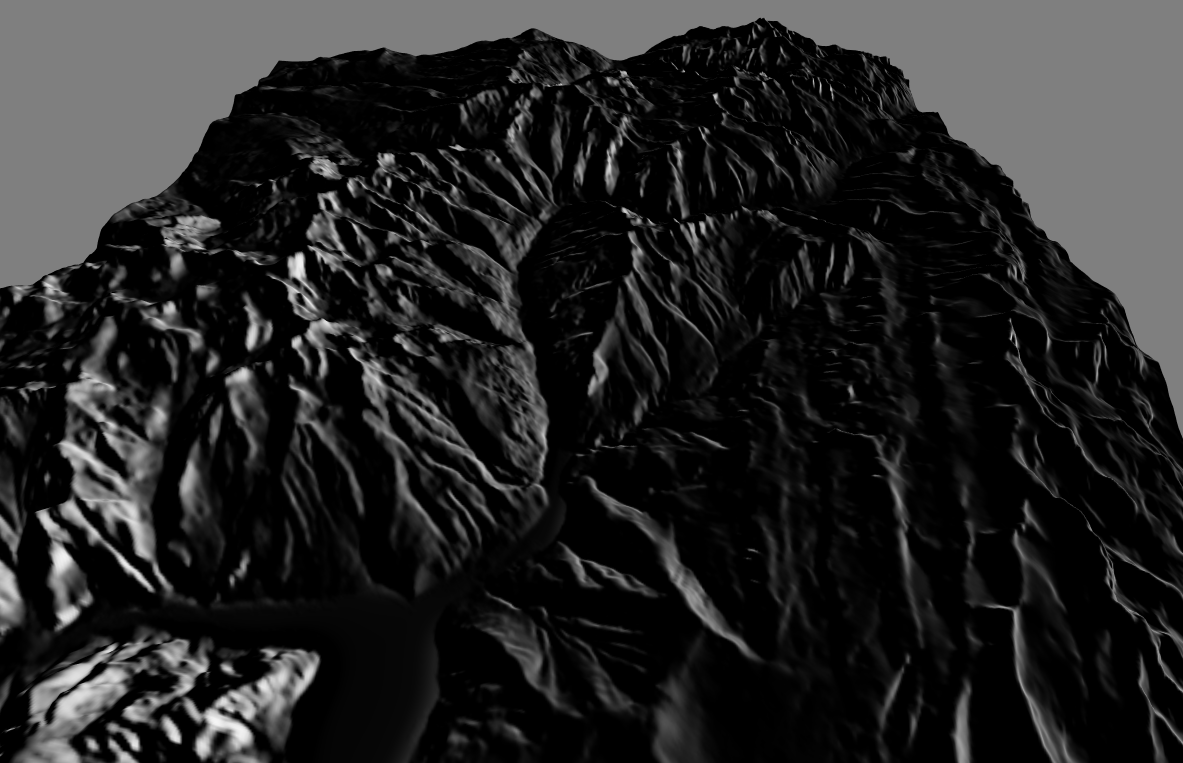
\includegraphics[width=1.0\linewidth]{Resultats/3_our_5.png}
   \caption{$\gamma_o = 5\degres$)}
 \end{subfigure}
 \begin{subfigure}[t]{0.24\linewidth}
   \centering
   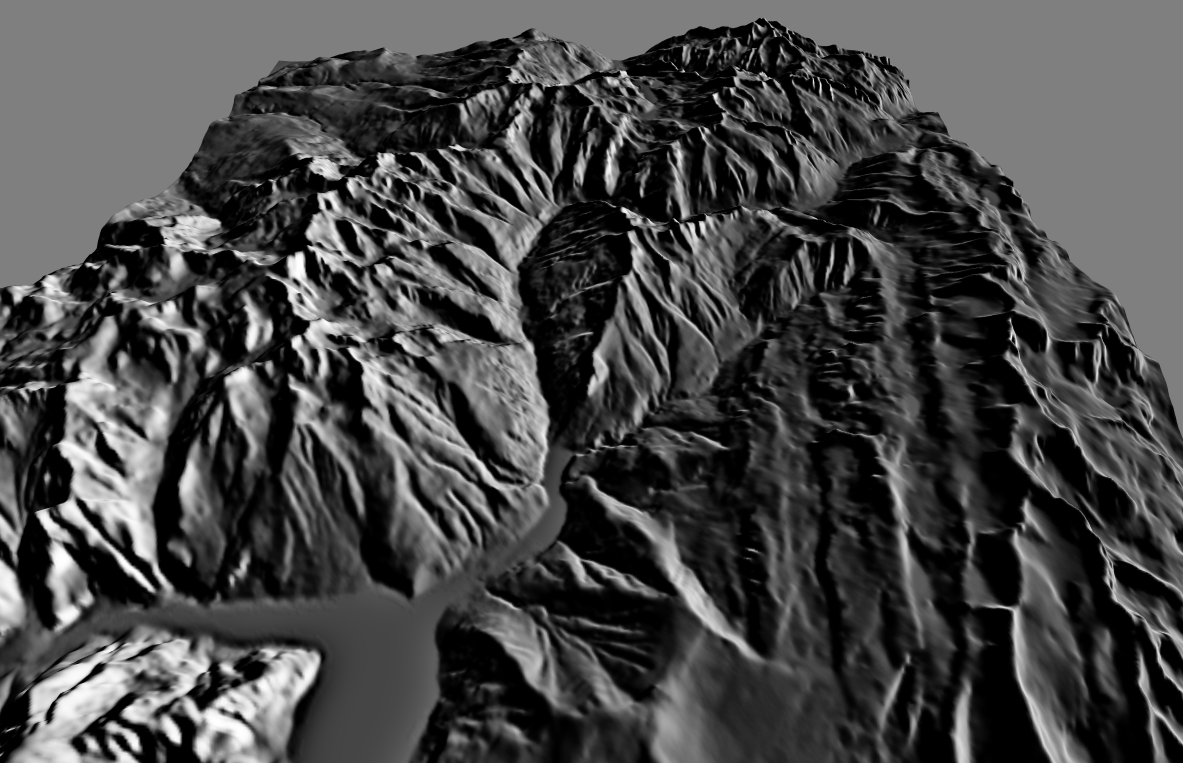
\includegraphics[width=1.0\linewidth]{Resultats/3_our_20.png}
   \caption{$\gamma_o = 20\degres$}
 \end{subfigure}
 \begin{subfigure}[t]{0.24\linewidth}
   \centering
   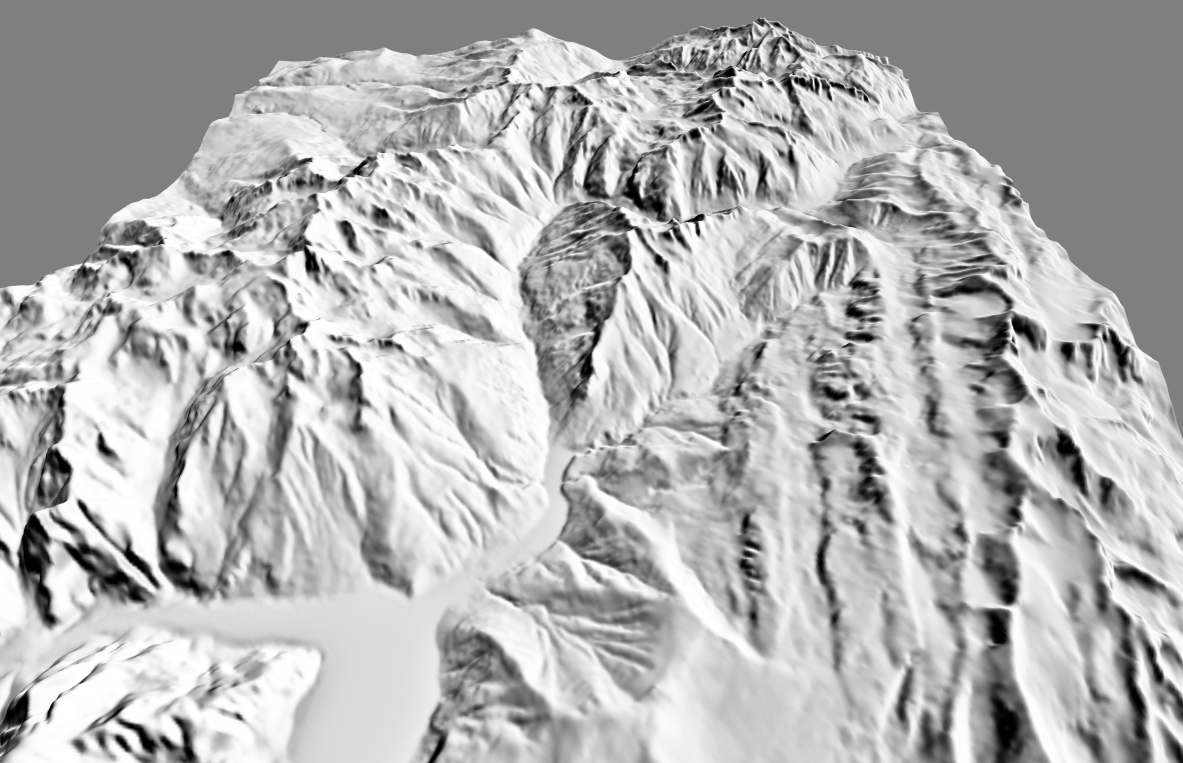
\includegraphics[width=1.0\linewidth]{Resultats/3_our_50.png}
   \caption{$\gamma_o = 50\degres$}
 \end{subfigure}
 \begin{subfigure}[t]{0.24\linewidth}
   \centering
   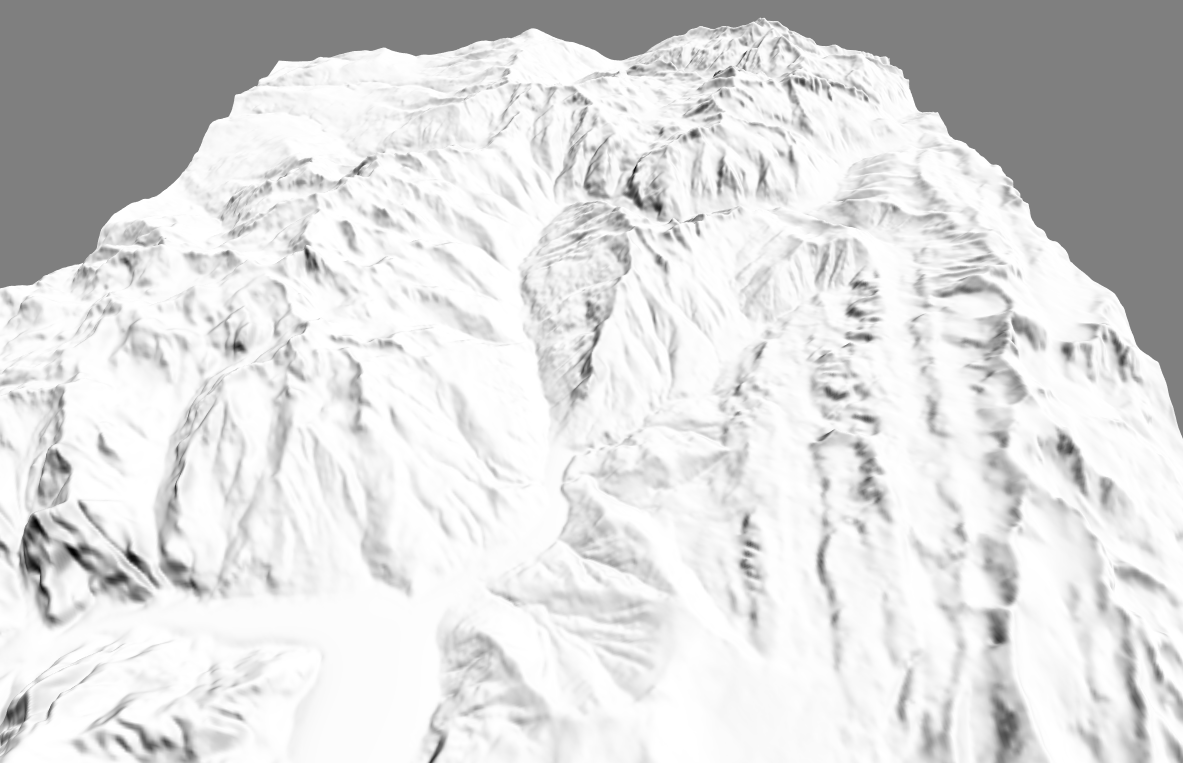
\includegraphics[width=1.0\linewidth]{Resultats/3_our_70.png}
   \caption{$\gamma_o = 70\degres$}
 \end{subfigure}
  \begin{subfigure}[t]{0.24\linewidth}
   \centering
   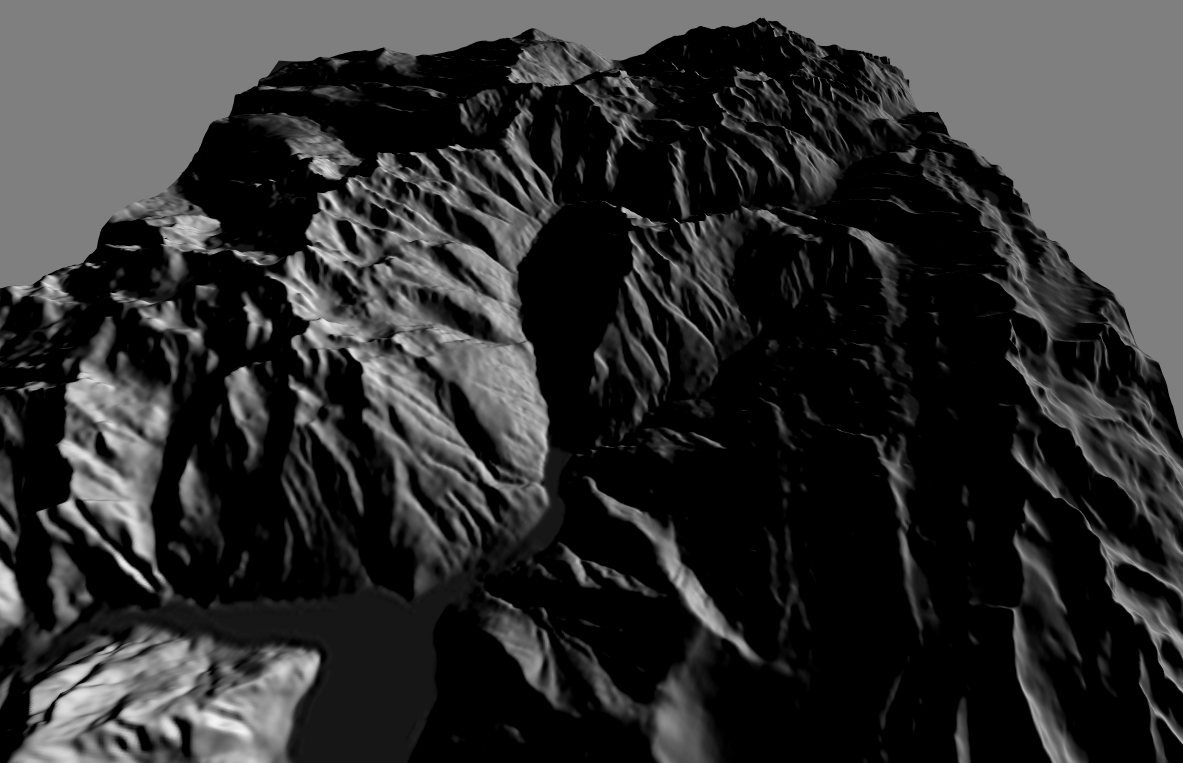
\includegraphics[width=1.0\linewidth]{Resultats/3_lambert_5.png}
   \caption{$\gamma_o = 5\degres$}
 \end{subfigure}
 \begin{subfigure}[t]{0.24\linewidth}
   \centering
   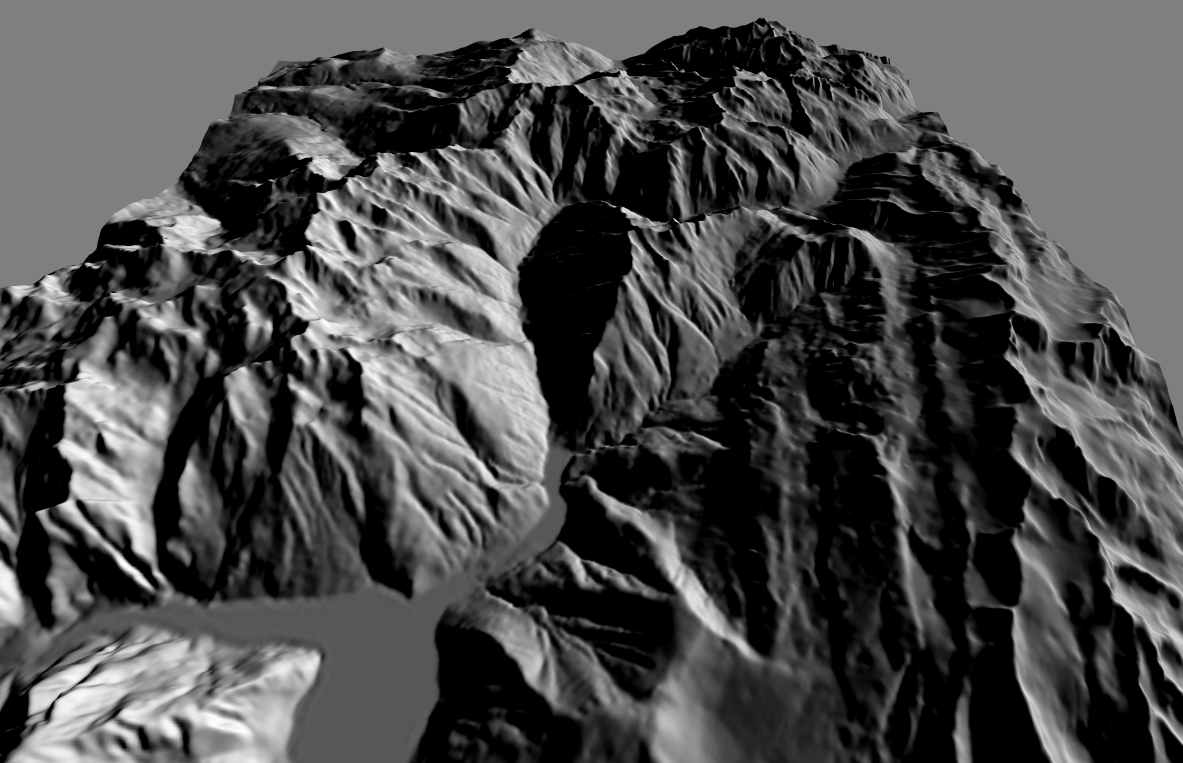
\includegraphics[width=1.0\linewidth]{Resultats/3_lambert_20.png}
   \caption{$\gamma_o = 20\degres$}
 \end{subfigure}
 \begin{subfigure}[t]{0.24\linewidth}
   \centering
   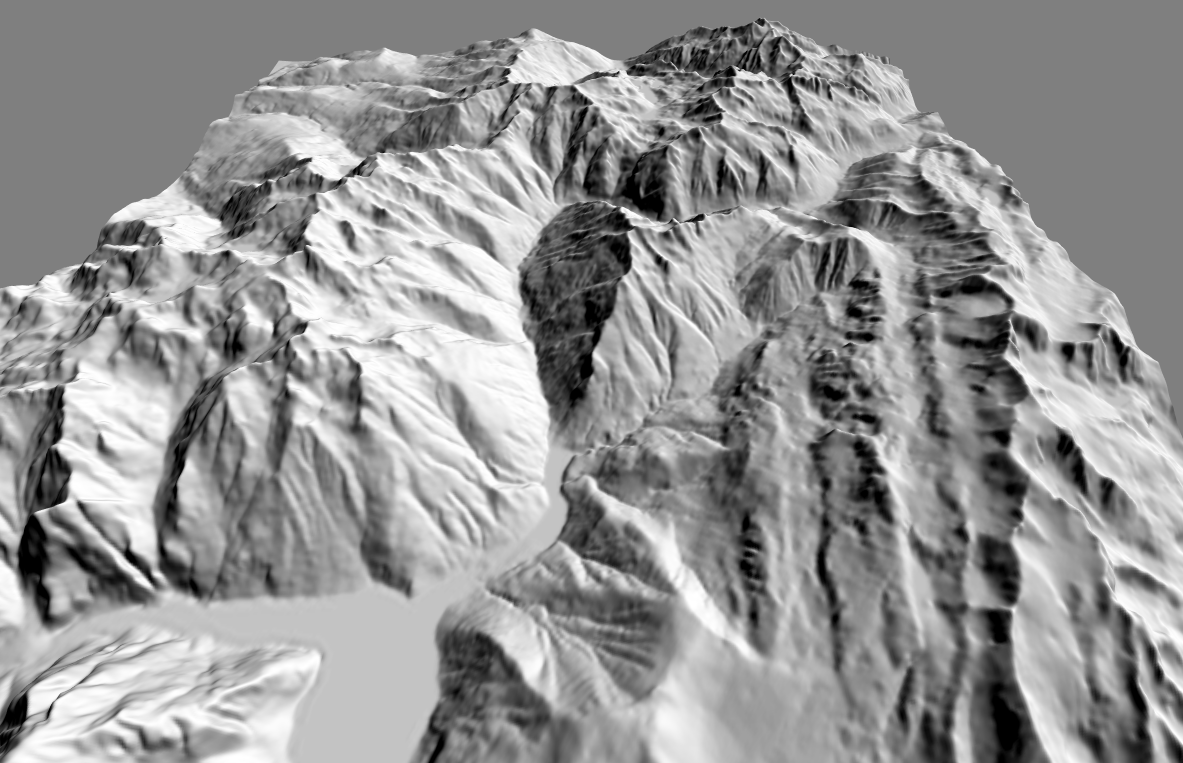
\includegraphics[width=1.0\linewidth]{Resultats/3_lambert_50.png}
   \caption{$\gamma_o = 50\degres$}
 \end{subfigure}
 \begin{subfigure}[t]{0.24\linewidth}
   \centering
   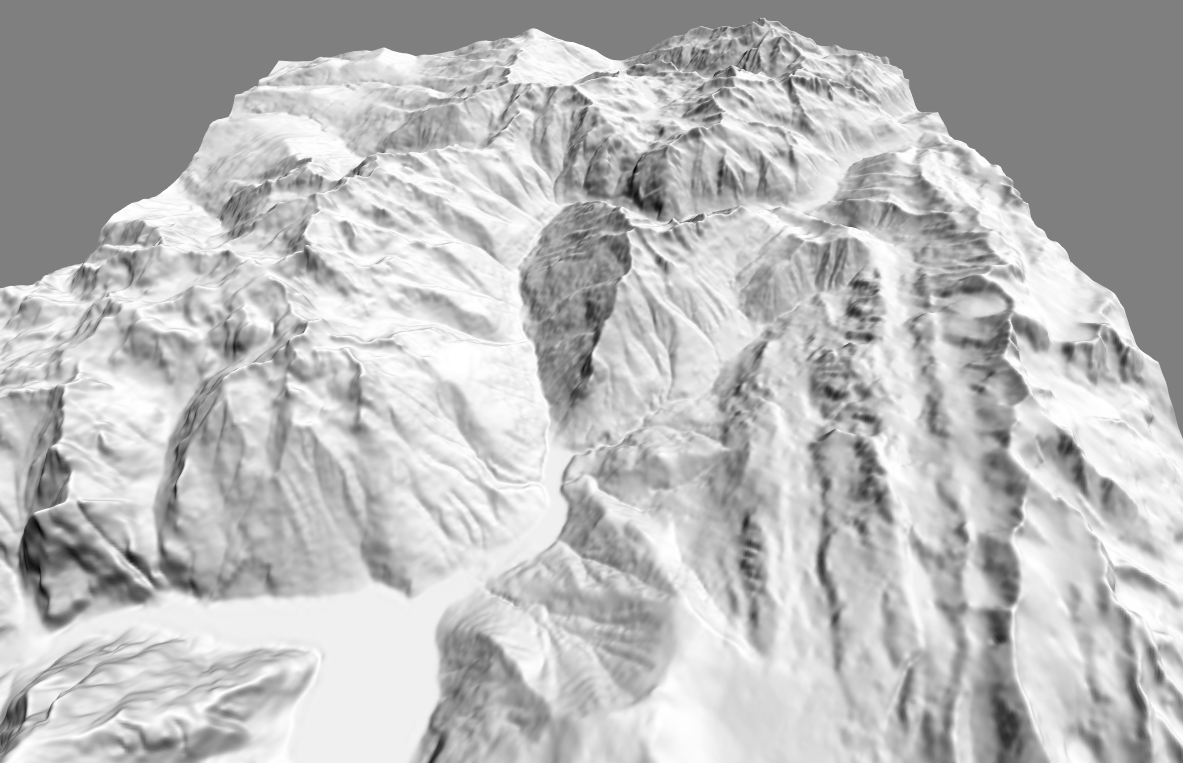
\includegraphics[width=1.0\linewidth]{Resultats/3_lambert_70.png}
   \caption{$\gamma_o = 70\degres$}
 \end{subfigure}
 \caption{Comparaison entre notre méthode (ligne du haut) et un Lambertien classique (ligne du bas) avec plusieurs élévations du Soleil ( $\alpha = 270\degres$ (Est) , $\sigma = 30$). }
\end{figure*}



\begin{figure*}[h!]
\centering
 \begin{subfigure}[t]{0.24\linewidth}
   \centering
   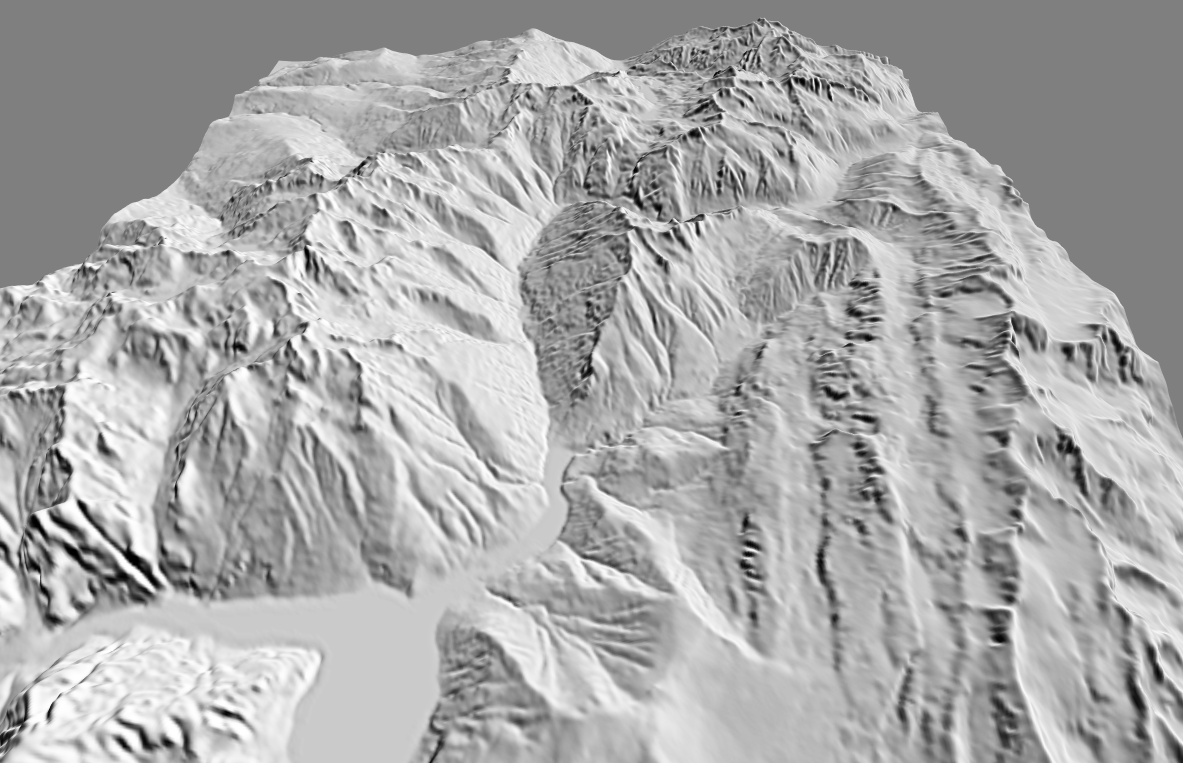
\includegraphics[width=1.0\linewidth]{Resultats/4_our_5.png}
   \caption{$\sigma = 5$}
 \end{subfigure}
 \begin{subfigure}[t]{0.24\linewidth}
   \centering
   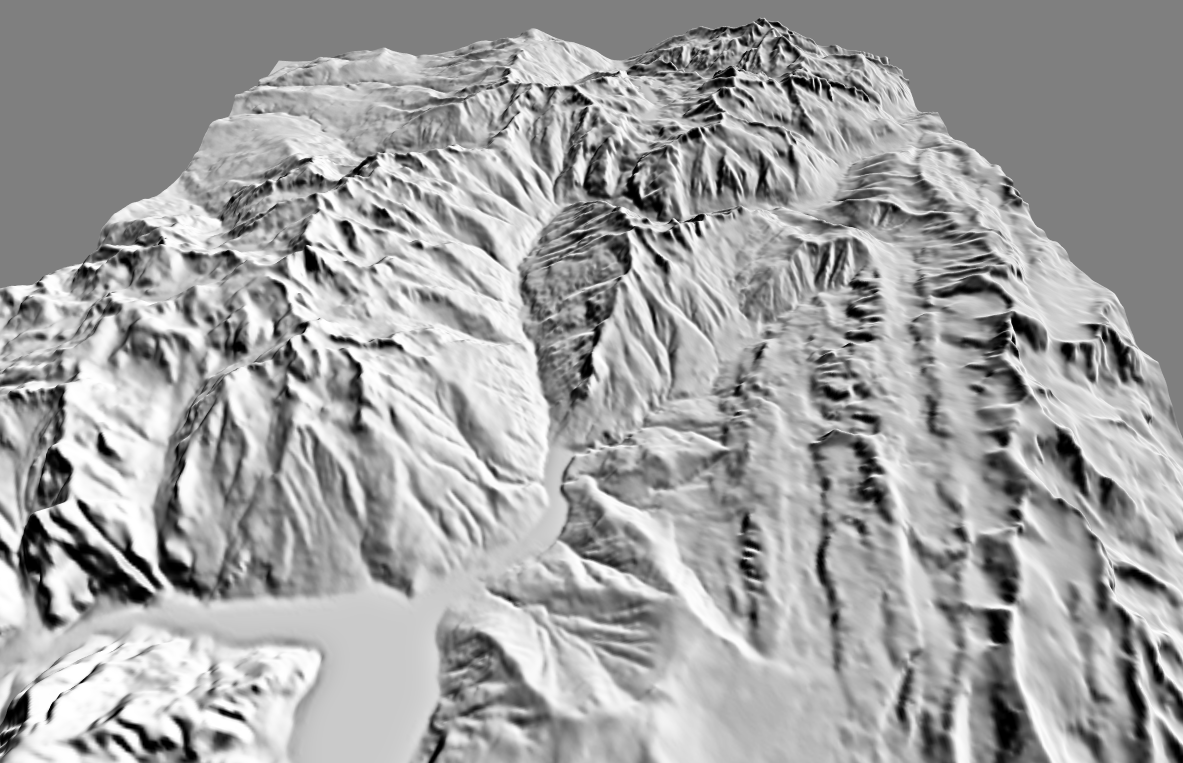
\includegraphics[width=1.0\linewidth]{Resultats/4_our_20.png}
   \caption{$\sigma = 20$}
 \end{subfigure}
 \begin{subfigure}[t]{0.24\linewidth}
   \centering
   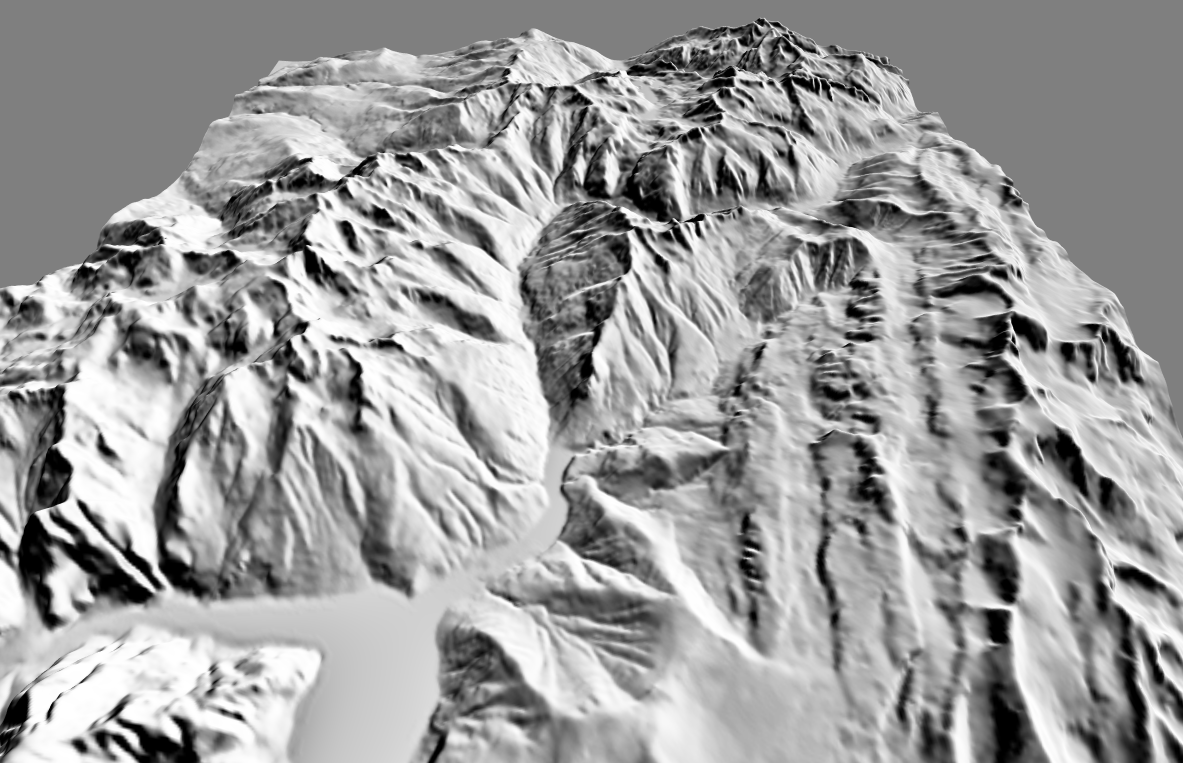
\includegraphics[width=1.0\linewidth]{Resultats/4_our_50.png}
   \caption{$\sigma = 50$}
 \end{subfigure}
 \begin{subfigure}[t]{0.24\linewidth}
   \centering
   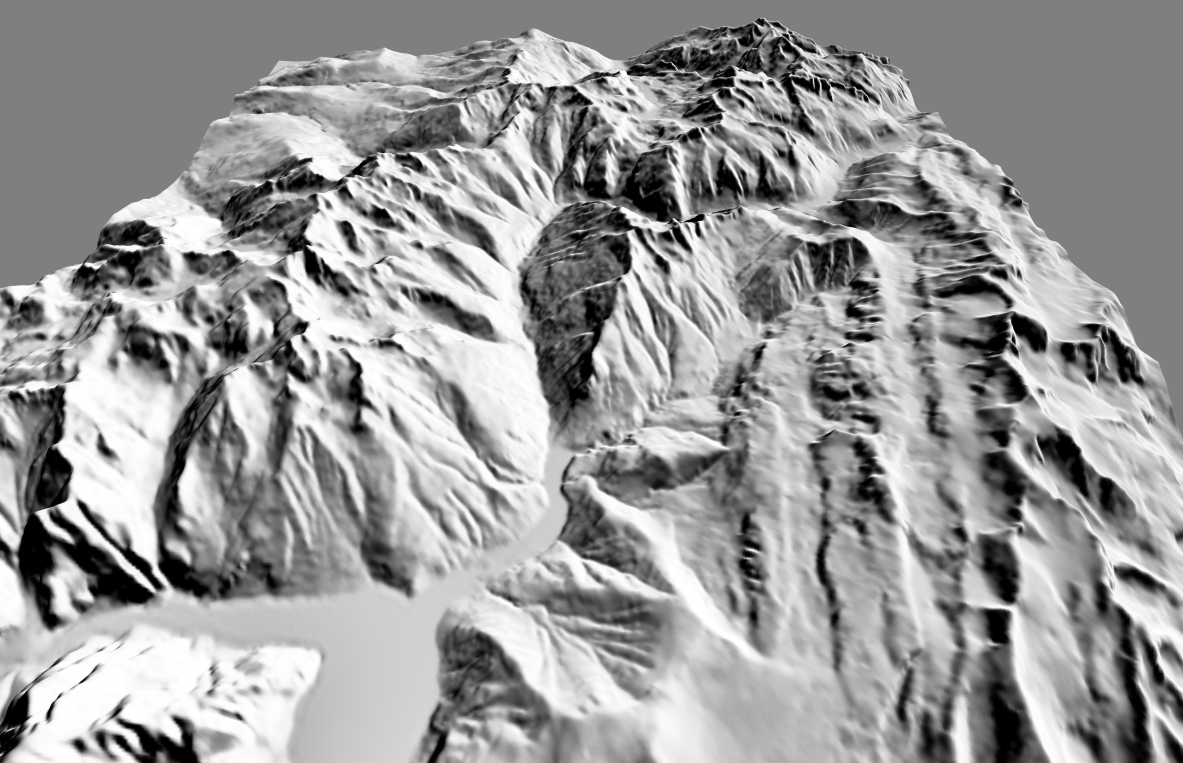
\includegraphics[width=1.0\linewidth]{Resultats/4_our_100.png}
   \caption{$\sigma = 100$}
 \end{subfigure}
 \caption{Comparaison entre plusieurs niveaux de flou ($\alpha = 315\degres$ (Nord-Est), $\gamma_o = 45\degres$).}
\end{figure*}

\begin{figure*}[h!]
\centering
 \begin{subfigure}[t]{0.49\linewidth}
   \centering
   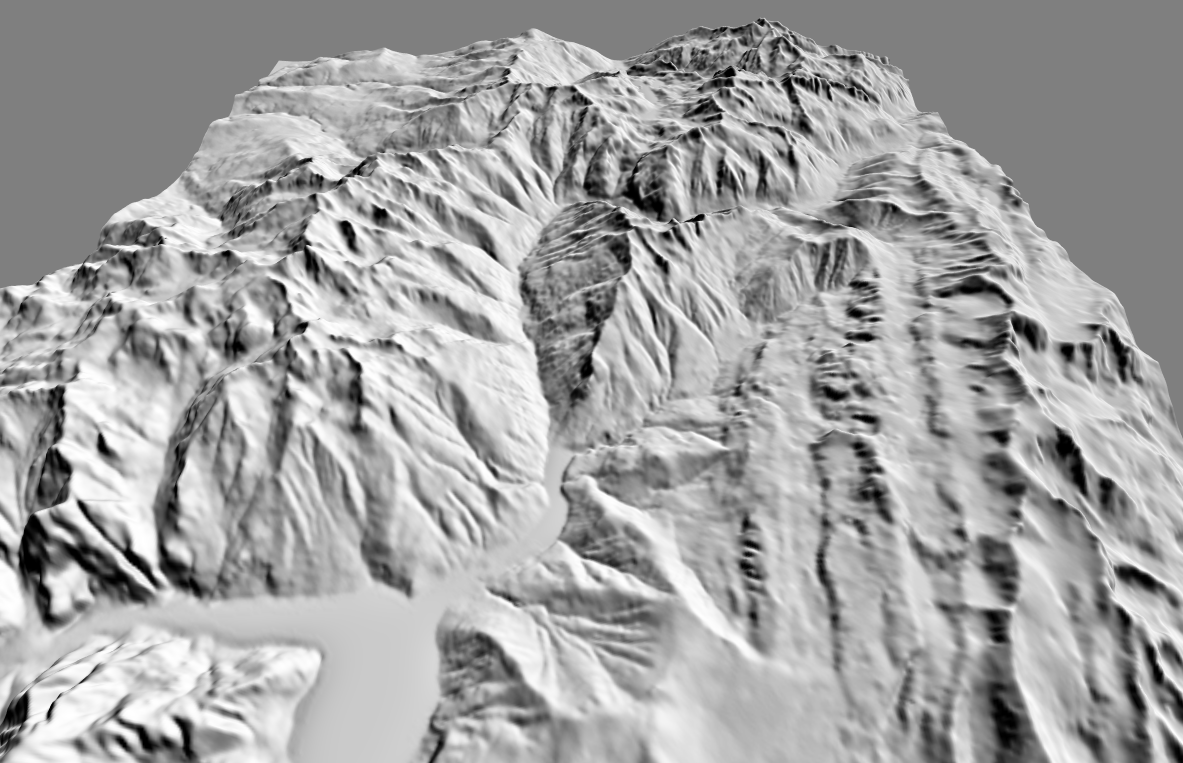
\includegraphics[width=1.0\linewidth]{Resultats/5_our_nonorien.png}
   \caption{Sans orientation}
 \end{subfigure}
 \begin{subfigure}[t]{0.49\linewidth}
   \centering
   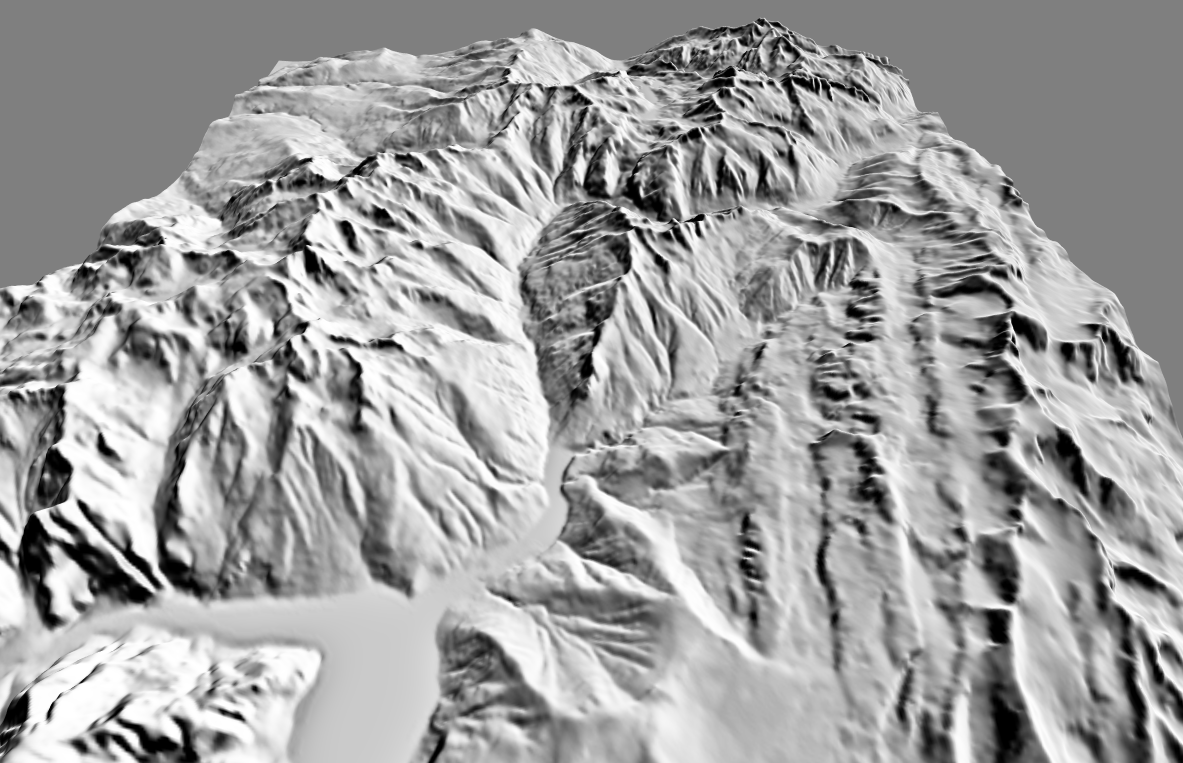
\includegraphics[width=1.0\linewidth]{Resultats/5_our_orien.png}
   \caption{Avec orientation}
 \end{subfigure}
 \caption{Comparaison avec et sans l'orientation de la lumière mais avec le multi-échelle ($\alpha = 315\degres$(Nord-Est), $\gamma_o = 45\degres$ , $\sigma = 30$).}
\end{figure*}

\begin{figure*}[h!]
\centering
 \begin{subfigure}[t]{0.32\linewidth}
 \centering
 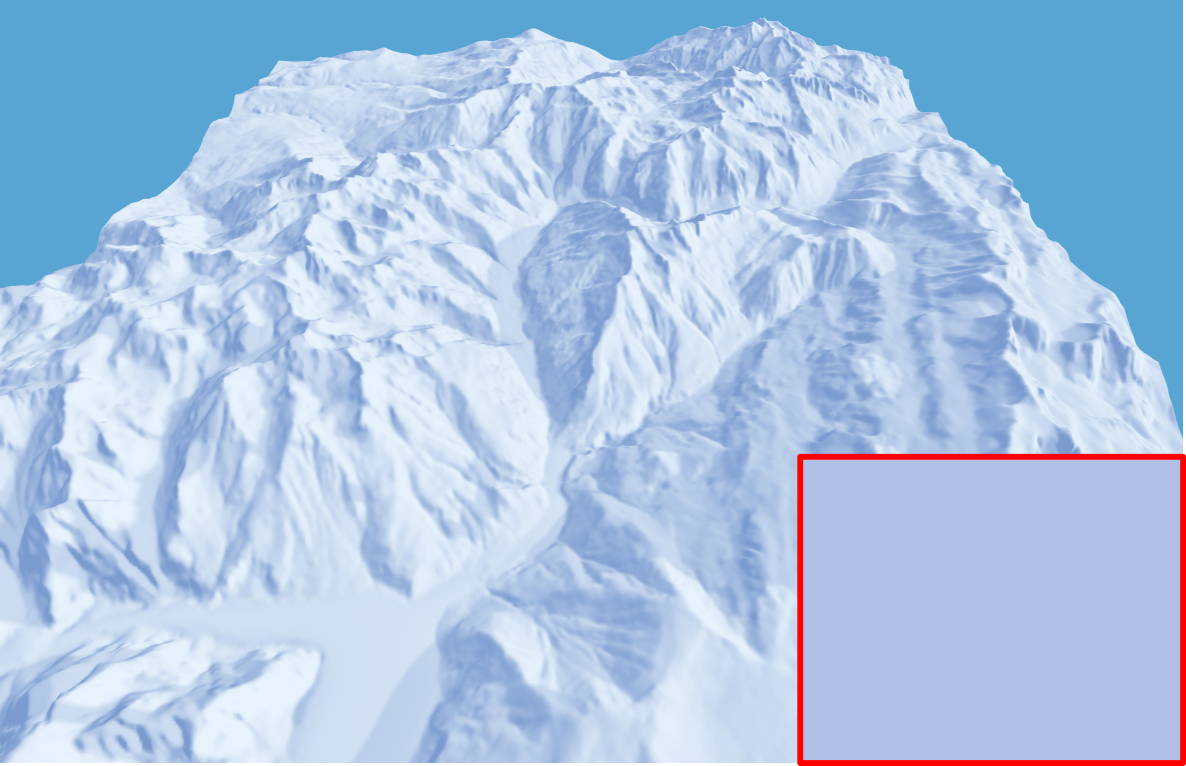
\includegraphics[width=1.0\linewidth]{Resultats/aquarelle.png}
 \caption{Aquarelle}
 \end{subfigure}
 \begin{subfigure}[t]{0.32\linewidth}
 \centering
 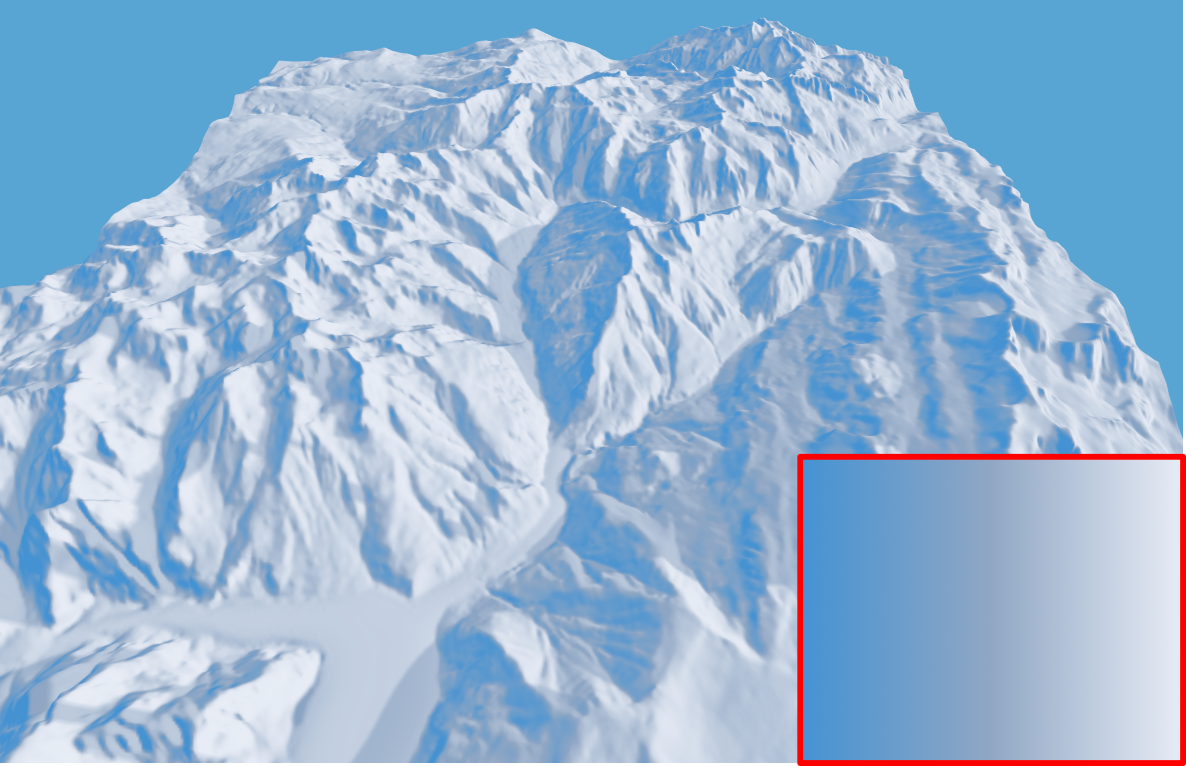
\includegraphics[width=1.0\linewidth]{Resultats/colorMap.png}
  \caption{\label{fig:degradeColor}Rampe de couleur dégradé}
 \end{subfigure}
  \begin{subfigure}[t]{0.32\linewidth}
 \centering
 
\includegraphics[width=1.0\linewidth]{Resultats/cel_shading.png}
  \caption{Cel-shading}
 \end{subfigure}
 \caption{\label{fig:colorOmbre} Comparaison des méthodes de colorisation avec des couleurs données par Arthur Novat($\alpha = 270\degres$ (Est) $\gamma_o = 45\degres$ , $\gamma_p = 20\degres$, $\sigma = 30$). }
\end{figure*}


\begin{figure*}[h!]
\centering
 \begin{subfigure}[t]{0.49\linewidth}
   \centering
   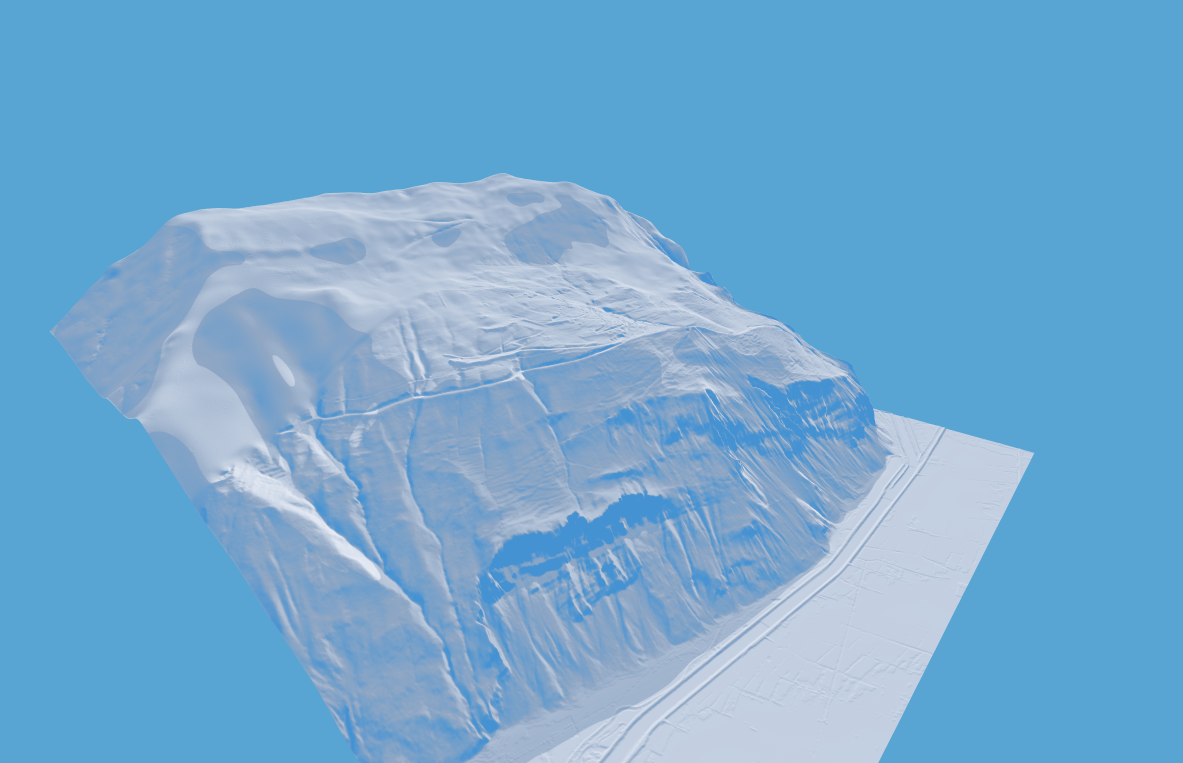
\includegraphics[width=1.0\linewidth]{Resultats/7_high_1.png}
   \caption{$\alpha = 45\degres$ (Nord-Ouest)}
 \end{subfigure}
 \begin{subfigure}[t]{0.49\linewidth}
   \centering
   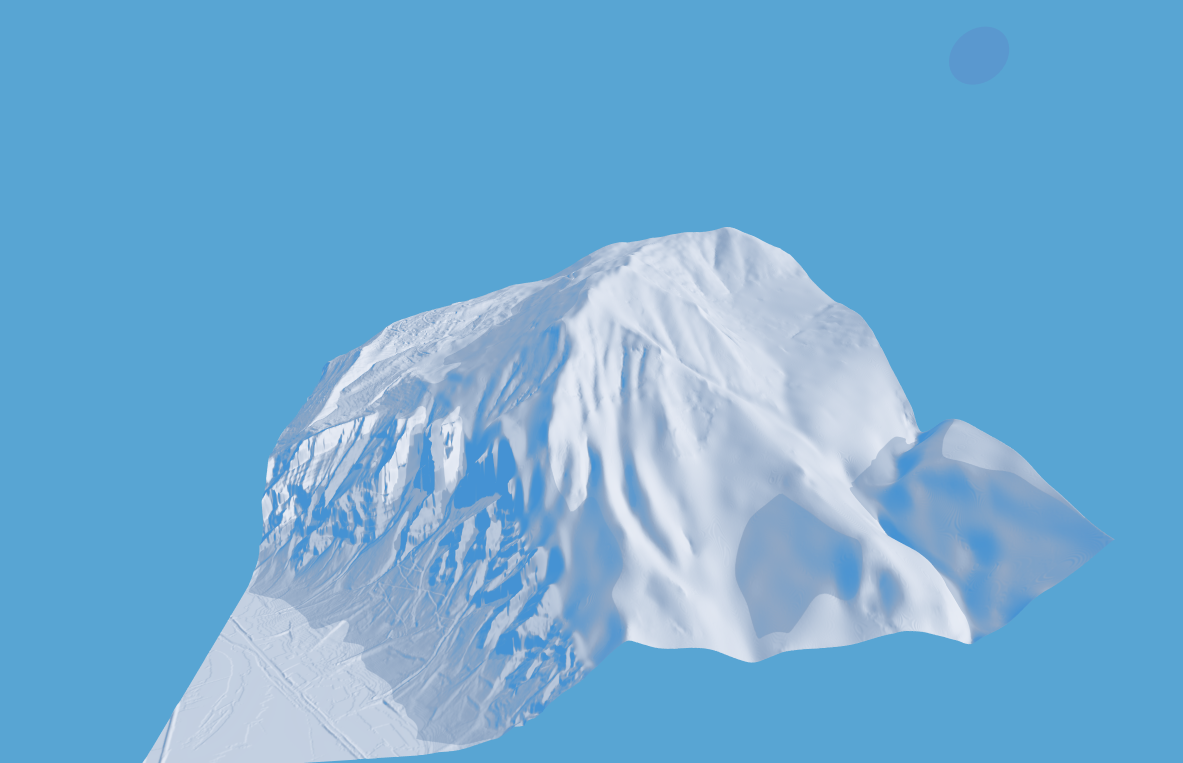
\includegraphics[width=1.0\linewidth]{Resultats/7_high_2.png}
   \caption{$\alpha = 270\degres$ (Est)}
 \end{subfigure}
 \caption{Terrain avec une résolution de $1$m ($\gamma_o = 45\degres$ , $\gamma_p = 30\degres$, $\sigma = 100$).}
\end{figure*}

\begin{figure*}[h!]

   \centering
   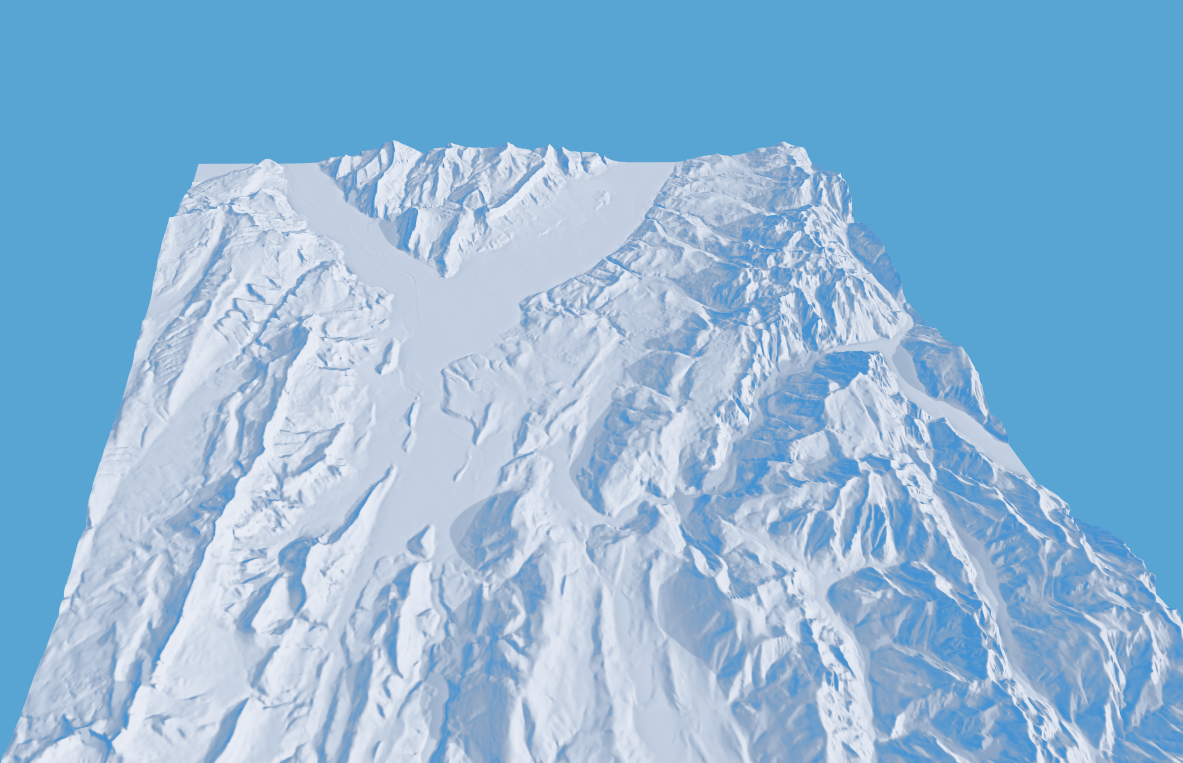
\includegraphics[width=1.0\linewidth]{Resultats/7_grenoble.png}
   \caption{Vallée de Grenoble colorisée avec la même rampe de couleur que la Figure \ref{fig:degradeColor} ($\alpha = 270\degres$ (Est) $\gamma_o = 45\degres$ , $\gamma_p = 20\degres$, $\sigma = 30$).}
\end{figure*}





